\documentclass[a4,useAMS,usenatbib,usegraphicx,12pt]{article}
%External Packages and personalized macros
%=========================================================================
%		EXTERNAL PACKAGES
%=========================================================================
\usepackage[round]{natbib}
\usepackage[margin=3cm]{geometry}
\usepackage{hyperref}
\usepackage{times}
\usepackage{amsmath} 
\usepackage{amssymb}
\usepackage{graphicx}
\usepackage{array, xcolor, lipsum, bibentry}
\usepackage[nottoc, notlof, notlot]{tocbibind}

\definecolor{lightgray}{gray}{0.8}
\newcolumntype{L}{>{\raggedleft}p{0.14\textwidth}}
\newcolumntype{R}{p{0.8\textwidth}}
\newcommand\VRule{\color{lightgray}\vrule width 0.5pt}

\usepackage{booktabs}% http://ctan.org/pkg/booktabs
\newcommand{\tabitem}{~~\llap{\textbullet}~~}

%=========================================================================
%		INTERNAL MACROS
%=========================================================================
% To highlight comments 
\definecolor{red}{rgb}{1,0.0,0.0}
\newcommand{\red}{\color{red}}
\definecolor{darkgreen}{rgb}{0.0,0.5,0.0}
\newcommand{\SRK}[1]{\textcolor{darkgreen}{\bf SRK: \textit{#1}}}
\newcommand{\SRKED}[1]{\textcolor{darkgreen}{\bf #1}}

\newcommand{\LCDM}{$\Lambda$CDM~}
\newcommand{\beq}{\begin{eqnarray}}  
\newcommand{\eeq}{\end{eqnarray}}  
\newcommand{\zz}{$z\sim 3$} 
\newcommand{\apj}{ApJ}  
\newcommand{\apjs}{ApJS}  
\newcommand{\apjl}{ApJL}  
\newcommand{\aj}{AJ}  
\newcommand{\mnras}{MNRAS}  
\newcommand{\mnrassub}{MNRAS accepted}  
\newcommand{\aap}{A\&A}  
\newcommand{\aaps}{A\&AS}  
\newcommand{\araa}{ARA\&A}  
\newcommand{\nat}{Nature}  
\newcommand{\physrep}{PhR}
\newcommand{\pasp}{PASP}    
\newcommand{\pasj}{PASJ}    
\newcommand{\avg}[1]{\langle{#1}\rangle}  
\newcommand{\ly}{{\ifmmode{{\rm Ly}\alpha}\else{Ly$\alpha$}\fi}}
\newcommand{\hMpc}{{\ifmmode{h^{-1}{\rm Mpc}}\else{$h^{-1}$Mpc }\fi}}  
\newcommand{\hGpc}{{\ifmmode{h^{-1}{\rm Gpc}}\else{$h^{-1}$Gpc }\fi}}  
\newcommand{\hmpc}{{\ifmmode{h^{-1}{\rm Mpc}}\else{$h^{-1}$Mpc }\fi}}  
\newcommand{\hkpc}{{\ifmmode{h^{-1}{\rm kpc}}\else{$h^{-1}$kpc }\fi}}  
\newcommand{\hMsun}{{\ifmmode{h^{-1}{\rm {M_{\odot}}}}\else{$h^{-1}{\rm{M_{\odot}}}$}\fi}}  
\newcommand{\hmsun}{{\ifmmode{h^{-1}{\rm {M_{\odot}}}}\else{$h^{-1}{\rm{M_{\odot}}}$}\fi}}  
\newcommand{\Msun}{{\ifmmode{{\rm {M_{\odot}}}}\else{${\rm{M_{\odot}}}$}\fi}}  
\newcommand{\msun}{{\ifmmode{{\rm {M_{\odot}}}}\else{${\rm{M_{\odot}}}$}\fi}}  
\newcommand{\lya}{{Lyman$\alpha$~}}
\newcommand{\clara}{{\texttt{CLARA}}~}
\newcommand{\rand}{{\ifmmode{{\mathcal{R}}}\else{${\mathcal{R}}$ }\fi}}  


%MY COMMANDS #############################################################
\newcommand{\sub}[1]{\mbox{\scriptsize{#1}}}
\newcommand{\dtot}[2]{ \frac{ d #1 }{d #2} }
\newcommand{\dpar}[2]{ \frac{ \partial #1 }{\partial #2} }
\newcommand{\pr}[1]{ \left( #1 \right) }
\newcommand{\corc}[1]{ \left[ #1 \right] }
\newcommand{\lla}[1]{ \left\{ #1 \right\} }
\newcommand{\bds}[1]{\boldsymbol{ #1 }}
\newcommand{\oiint}{\displaystyle\bigcirc\!\!\!\!\!\!\!\!\int\!\!\!\!\!\int}
\newcommand{\mathsize}[2]{\mbox{\fontsize{#1}{#1}\selectfont $#2$}}
\newcommand{\eq}[2]{\begin{equation} \label{eq:#1} #2 \end{equation}}
\newcommand{\lth}{$\lambda_{th}$ }
%#########################################################################

\setlength\parindent{0pt}
 
\title{{\textbf{Research Proposal for DAAD PhD scholarship}}\\ The Gaseous Cosmic Web with AREPO\\ \color{black}\rule{15cm}{0.5mm}}
\author{Sebastian Bustamante Jaramillo}
\date{}
  
\begin{document}
\maketitle
\begin{center}
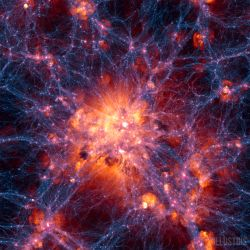
\includegraphics[trim = 0mm 3.5cm 0mm 3.0cm, clip, keepaspectratio=true,
width=0.7\textheight]{Presentation1.png}
\tiny{A projection of the cosmic web in the ILLUSTRIS simulation, that was made 
with AREPO (http://www.illustris-project.org/)}
\end{center}
\tableofcontents
 
\newpage 

%============================================================================== 
\section{General Information}
\small
\subsection*{Information of the Applicant}
\begin{tabular}{L!{\VRule}R}
\bf Name		& Sebastian Bustamante Jaramillo\\
\bf Degree		& B.Sc. in Physics, Universidad de Antioquia (2013)\\
\bf Position	& Adjunct Professor, Universidad de Antioquia\\
\bf Birthday	& { 20$^{th}$ June, 1990}\\
\bf Nationality & Colombian\\
\bf ID			& C.C. 1128400433\\
\bf Address 1	& Avenida 21 \# 57 AA 65, Bello - Colombia (personal)\\
\bf Address 2	& Calle 67 \# 53 - 108, Off. 5-330, Medellin, Colombia (work)\\
\bf Phone		& +057 (4) 4820138\\
\bf Mobile		& +057 3108992409\\
\bf E-mail 1	& macsebas33 \textit{at} gmail.com (personal)\\
\bf E-mail 2	& sebastian.bustamante \textit{at} udea.edu.co (academic)\\
\end{tabular}

\vspace{10pt}

More detailed information of the applicant can be found here \url{http://goo.gl/BPZGzK}

\vspace{15pt}  

\subsection*{Information of the Project}
\begin{tabular}{L!{\VRule}R}
\bf Title		& \bf The Gaseous Cosmic Web with AREPO\\
\bf Field		& Cosmology, Astrophysics, Physical Sciences \\
\bf Advisor 1	& Volker Springel, PhD. Heidelberg Institute for Theoretical Studies (HITS) \& University of Heidelberg, Germany \\
\bf Advisor 2	& Jaime Forero-Romero, PhD. Universidad de los Andes, Colombia \\
\bf University	& University of Heidelberg, IMPRS PhD program \\
\bf Time Frame	& 3 years \\
\end{tabular}
\normalsize
%==============================================================================

\newpage

%==============================================================================
\section{Introduction}


The filamentary nature of the large-scale matter distribution (the so-called 
cosmic web) is one of the most striking features of Universe \citep{Bond96}, 
being an essential part of the current standard paradigm in cosmology. Last 
generation galaxy redshift surveys, such as the \textit{two-degree-Field Galaxy 
Redshift Survey} (2dFGRS, see \citet{Colless03}) and the \textit{Sloan Digital 
Sky Survey} (SDSS, see \citet{Abazajian09}), reveal the cosmic web at a level 
of detail never seen before. In addition, other observational probes like the 
Ly-$\alpha$ forest in distant quasars \citep{Rauch98, Cantalupo14}, 
fluorescence emissions \citep{Cantalupo12} and weak gravitational lensing 
\citep{Massey07, Dietrich12} have also validated this picture undoubtedly.

\

On the theoretical side, early descriptions of the evolution of the large-scale
Universe, based on gravitational instabilities in primordial stages and leaded 
by the seminal work of \citet{Zeldovich70}, predict the cosmic web picture. 
Since then, our understanding of the structure and dynamics of the cosmic web 
has been dramatically improved as new and more powerful theoretical and 
computational tools and better observational data become available. In 
particular, N-body simulations, fuelled by last generation computing systems 
and ever more efficient numerical algorithms, have an increasingly important 
role in revealing the complexity of the large-scale Universe.

\

In the current cosmological paradigm, the $\Lambda$CDM model, there are two 
different types of matter, i.e. baryonic or luminous matter, corresponding 
to what we can see, and the poorly interacting (and of a still unknown nature) 
dark matter. The most actual measurements of their abundances indicate a 
proportion approximately of 1 to 6, respectively \citep{Planck13XVI}. 
Accordingly, most of the related numerical research has been made based on 
dark matter-only N-body simulations, where the gas dynamics has been 
neglected (for a very detailed numerical analysis of the dark matter cosmic 
web, see \citet{Cautun14}). Nevertheless, recent simulation studies in 
filamentary gas accretion in high redsfhit galaxies \citep{Dekel09}, 
large-scale orientation and alignment of the spin of galaxies with they 
embedding cosmic web \citep{Hahn10}, and filamentary-induced exchange of 
galaxy angular momentum \citep{Dubois14}, have proven the need of using 
fully hydrodynamical cosmological simulations due to the high level of coupling
between dark and baryonic matter.

\

Incorporating gas dynamics into cosmological simulations is far from an easy 
task. The first reason is the highly complex \textit{gastrophysical} processes 
involved in baryonic dynamics, i.e. shock heating, photoionization, supernova 
feedback, stellar wind, radiative cooling, star formation \citep{Bond93}. The
second reason is the complexity of the hydrodynamical equations followed by 
the gas. Traditionally, two different hydro-solvers have been used for this 
task, i.e. a Lagrangian \textit{Smoothed Particle Hydrodynamics} (\texttt{SPH}) 
technique \citep{Monaghan92} (for an implementation, see e.g. the \texttt{GADGET} 
code by \citet{Springel05}) and an Eulerian solver on a mesh with \textit{
Adaptive Mesh Refinement} (\texttt{AMR}) \citep{Berger89} (for an implementation, 
see e.g. the \texttt{RAMSES} code by \citet{Teyssier02}). 

\

The \texttt{SPH} scheme is easily implemented on a computer due to its 
Lagrangian character. Furthermore, as the mesh follows the evolution of each 
single particle and has a continuously auto-adjusting resolution, its usage is 
very suitable for problems like turbulent flows. However, its same Lagrangian 
nature originates an inhomogeneous and distorted spatial resolution, what makes 
difficult to account for low density regions in simulations and causes 
suppressions in fluid instabilities, making it poor suitable for capturing shock
dynamics. An artificial viscosity term is usually introduced for improving the 
accuracy in these situations. On the other hand, \texttt{AMR} is more efficient 
for capturing shock dynamics. However, due to the conservative nature of the 
hydrodynamical equations, a fixed mesh causes a lack of Galilean invariance, 
making the computer implementation considerable harder. Furthermore, the 
unsmooth sampling of physical properties introduces spurious vorticity to the 
fluid, making the scheme unsuitable for studying turbulent flows (for a further
discussion and comparison of both schemes, see \citet{Plewa01}).

\

Recently, a completely new paradigm was introduced by \citet{Springel10} and 
implemented in the \texttt{AREPO} code. It combines the strengths of 
\texttt{AMR} and \texttt{SPH} but overcoming their weaknesses. This code uses 
a moving mesh based on a Voronoi tessellation defined over a set of particles
that represents the fluid. The geometry of the mesh resembles very closely that 
of the point distribution, avoiding a distorted spatial resolution and retaining 
the auto-adaptivity inherent of \texttt{SPH}. Unlike \texttt{AMR}, the 
hydro-solver of \texttt{AREPO} is based on a Gudonov's scheme that guarantees the
Galilean invariance and the conservative nature of the solutions. All of these 
features makes \texttt{AREPO} highly efficient and accurate for simulating a 
plethora of hydrodynamical problems, even including those where \texttt{AMR} and
\texttt{SPH} fail separately. Hence \texttt{AREPO} is a very attractive approach 
for computing fully hydrodynamical simulations of the large-scale Universe.



%==============================================================================

\newpage
%==============================================================================
\section{Objectives}
%==============================================================================


\begin{itemize}

\item[\checkmark] Study gaseous filamentary accretion of the cosmic web using 
\texttt{AREPO} simulations.

\item[\checkmark] Quantify the impact of gaseous filamentary accretion on galaxy 
evolution.

\item[\checkmark] Deriving observable quantities from our theoretical studies.


\end{itemize}



%==============================================================================
\section{Methodology}
%==============================================================================


The proposed project is subject to a PhD study and will cover the following 
aspects:

\

\begin{itemize}

\item[\checkmark] \textit{First, an analysis and characterization of existing 
hydrodynamical simulations based on the \texttt{AREPO} code will be done.}

\end{itemize}

As this project will be entirely based on numerical results, an analysis and 
characterization of existing \texttt{AREPO} hydrodynamical simulations is one 
of the key steps; the achieved unprecedented accuracy will guarantee a proper 
description of the simulated Universe.


This step includes a quantification of the dark matter and the gaseous cosmic
web through two different web finding schemes (i.e. the T-web based on the 
tidal tensor \citep{Hahn07,Forero09}, and the V-web based on the velocity shear
tensor \citep{Hoffman12}, schemes in which prof. Jaime Forero-Romero has a wide 
research trajectory); thus voids, walls, filaments and clusters will be 
identified. Then, a statistical analysis of the found structures will be done, 
i.e. volume and mass filling fractions at different redshifts, morphology, halo 
populations and filamentary accretion of gas.

In Heidelberg, the required computer facilities and the access to existing 
\texttt{AREPO} simulations and the private code (of which Prof. Volker 
Springel is the main author) is granted. Moreover, the renowned research 
trajectory and the expertise of Prof. Springel in numerical cosmology is 
certainly another appealing for pursuing this specific PhD project.

\

\begin{itemize}

\item[\checkmark] \textit{Second, detailed simulations of specific process at
high redshifts will be computed.}

\end{itemize}


\

\begin{itemize}

\item[\checkmark] \textit{Third, once established the underlying dark matter 
cosmic web, it is necessary to quantify the through gas dynamics. To this aim, 
inward and outward gas flows through potential wells (set by non-linear 
structures such as clusters and filaments) and accretion rates of the gas 
component residing within dark matter halos at different redshifts should be 
computed. At this point, it should be possible to evaluate environmental
influences on different astrophysical phenomena. }

\end{itemize}


In order to exploit the new accuracy provided by the \texttt{AREPO} code, a 
correct quantification of the gas dynamics should be done. The current 
cosmological paradigm predicts a complex pipeline set by the potential well of 
non-linear structures, generally corresponding to clusters and filaments, 
through which the gas is transported toward over-dense regions like dark matter 
haloes. This process yields to different environmental phenomena of great current 
interest. We list here the most relevant for this project: influence of 
filament-induced flows on star forming galaxies at high redshifts, acquisition of 
the spin of galaxies through exchanging of angular momentum with the gaseous 
cosmic web, and kinematical and dynamical effects of the host environment on Local 
Group-like systems.



%==============================================================================
\section{Current State}
%==============================================================================


At present the applicant has already the fundamental basis in Astrophysics and
Cosmology required for this investigation. This can be confirmed by his research 
trajectory, including a paper (as co-author) published in \textit{ApJL} in which 
was studied the kinematics of the Local Group in a cosmological context, another 
paper (as co-author) published in \textit{ApJ} where was studied the influence 
of thermal evolution in the magnetic habitability of rocky planets, and some 
participations in academic congresses. Furthermore, a Bachelor's thesis
\footnote{Further information and an electronic version of this thesis can be 
found here \url{https://github.com/sbustamante/Thesis}.} where was studied the 
preferred place of simulated Local Group-like systems regarding the host 
environment in the cosmic web, also proves the ability of the applicant for 
handling simulations and massive data, a skill that is necessary for carrying 
out this project.

\

Currently, the applicant is involved in two research projects: first, a new 
method for finding voids in simulations based on the local fractional 
anisotropy. An ongoing publication (as first author) related to this is close 
to be submitted. \footnote{Information of this paper can be found here 
\url{https://github.com/sbustamante/CosmicVoidsPaper}.}. The second project is
about a comparison of three simulation techniques, i.e. \texttt{SPH} vs 
\texttt{VPH} vs \texttt{AREPO}, with possible publishable results at the end of
the present year.

%==============================================================================
\section{Timetable}
%==============================================================================

\begin{table}[h]
\begin{flushleft}
\begin{center}
  \begin{tabular}{l  l} \hline\hline
	\centering\textbf{Year} & \textbf{Goals} \\ \hline
	%First year
	First  
	& \tabitem First goal \\
	& \tabitem Second goal\\
	
	\\
	%Second year	
	Second
	& \tabitem First goal \\
	& \tabitem Second goal\\

	\\	
	%Third year	
	Third
	& \tabitem First goal \\
	& \tabitem Second goal\\ 
	
	\hline\hline
  \end{tabular}  
\end{center}
\end{flushleft}
\end{table}


%==============================================================================
\bibliographystyle{latex/mn2e}
\renewcommand{\bibname}{8\ \ \ \ Bibliography}
\bibliography{references.bib}
%==============================================================================



\end{document}